\documentclass[12pt]{article}
\usepackage[english]{babel}
\usepackage[utf8x]{inputenc}
\usepackage[T1]{fontenc}
\usepackage{scribe}
\usepackage{listings}
\usepackage{graphics, graphicx}
\usepackage{enumitem}
\usepackage{tcolorbox}
\usepackage{adjustbox}
\usepackage{amsmath,amssymb}
\usepackage{forest}
\usepackage{tikz}
\usetikzlibrary{positioning}
\graphicspath{ {./images/} }

\CourseName{Comtemporary Algorithms T.II/2019-20}
\Scribe{Pitipat Chairoj \& Nuttapat Koonarangsri}
\Lecturer{Kanat Tangwongsan}
\LectureNumber{2}
\LectureDate{8 January 2020}
\LectureTitle{Splay Tree and Treap}

\lstset{style=mystyle}

\newlist{steps}{enumerate}{1}
\setlist[steps, 1]{label = Step \arabic*:}

\begin{document}
\MakeScribeTop

%#############################################################
%#############################################################
%#############################################################
%#############################################################

\section{Splay Tree}

In a Binary Search Tree, root is a great position. Operations such as insert, delete, and join will be easier if
we promote a node to be the root. And, we can promote a node without violating BST rules. 

\textbf{Splay Tree} is a self-balancing binary search tree. A node in a splay tree will get promoted to the root of the tree, by using rotations, every time the
node is accessed.

However, promoting a node to be the root could be costly. Consider a binary search tree of $n$ nodes labeled from $0$ to $n-1$ with the node labeled $n-1$ as
the root and the node labeled $0$ being the leftmost node in the tree. With single rotations, if we
promote $0$, then $1$, then $2$, etc. sequentially, the total work is $\Omega(n^2)$ (with an amortized lower bound of $\Omega(n)$
per promotion). Splay tree do the rotation and restructuring in a very special way that guarantees
a logarithmic amortized bound.

\begin{figure}[h]
  \centering
  \includegraphics[scale=0.5]{promotion.png}
  \caption{Promotion (with single rotations)}
\end{figure}


\subsection{Rewrite Rules}
In the following rules, $x$ will be accessed, and we will apply rules until $x$ becomes the
Hello
root

\begin{enumerate}
    \item \begin{minipage}[t]{\linewidth}
              \raggedright
              \adjustbox{}{
                \includegraphics[scale=0.5]{zig.png}
              }
              \medskip

              Zig (single rotation)
        \end{minipage}
    \item \begin{minipage}[t]{\linewidth}
              \raggedright
              \adjustbox{}{
                \includegraphics[scale=0.5]{zig-zag.png}
              }
              \medskip

              Zig-Zag (double rotations)
        \end{minipage}
    \item \begin{minipage}[t]{\linewidth}
              \raggedright
              \adjustbox{}{%
                \includegraphics[scale=0.5]{zig-zig.png}
              }
              \medskip
              
              Zig-Zig (double rotations)
        \end{minipage}
\end{enumerate}

Note that each rule has a symmetric version. \textbf{splay(x)} refers to applying rewrite
rules to promote a node $x$ to be the root.

\begin{figure}[h]
  \centering
  \includegraphics[scale=0.5]{example-1.png}
  \caption{Splaying Example}
\end{figure}

\subsection{The Amortized Analysis}

\begin{tcolorbox}
\textbf{Recap: Potential Method}
$$ \text{Amortized cost} = \frac{\text{total cost of a sequence of operations}}{\text{total number
of operations}} $$
$$ \underbrace{\Phi(D)}_{\text{potential function}} = \text{reserve stored in data structure $D$ at
the point} $$
Let say $\sigma_1, \sigma_2, \dots, \sigma_m$ are operations performed on data structure $D$, and the
cost of operation $\sigma_i = c_i$
Initially, $D$ is at state $s_0$, and $\sigma_i$ changes state $s_{i-1} \rightarrow s_i$.
Then, the amortized cost of operation $\sigma_i$ is given by $$A_i = c_i + \Phi(s_i) -
\Phi(s_{i-1})$$
via summation:
\begin{align}
    \sum A_i = \sum c_i + \Phi(s_m) - \Phi(s_0)
\end{align}

Steps:
\begin{steps}[leftmargin=3cm]
 \item Choose a potential function.
 \item Prove that amortized cost satisfied the bound.
 \item Bound $\Phi(s_m) - \Phi(s_0)$ appropriately.
\end{steps}
\end{tcolorbox}

\begin{figure}[h]
    \centering
    \includegraphics[scale=0.5]{size-rank.png}
\end{figure}
      
Take any tree $T$. For a node $x \in T$, define
\begin{align*}
    s(x) &:= \text{number of nodes inside the subtree rooted at x}\\
    r(x) &:= \lfloor \text{log}_2(s(x)) \rfloor\\
    \Phi(T) &:= \sum_{x \in T} r(x) = \sum_{x \in T} \lfloor \text{log}_2(s(x)) \rfloor
\end{align*}

\paragraph{Example}
\begin{itemize}
    \item
        \begin{minipage}[t]{\linewidth}
              \raggedright
              \adjustbox{}{%
                \includegraphics[scale=0.5]{lopsided.png}
              }
              \medskip

              Lopsided tree: $\Phi \approx \sum_{k=1}^{n} \text{log}_2(k) \in \Theta(n\text{log}(n))$
        \end{minipage}
    \item
        \begin{minipage}[t]{\linewidth}
              \raggedright
              \adjustbox{}{%
                \includegraphics[scale=0.5]{pbst.png}
              }
              \medskip

              Perfect Binary Search tree: $\Phi \approx \sum_{i=0}^{\text{log}_2(n)} 2^i(\text{log}_2(n) - i) \in \Theta(n)$
        \end{minipage}
\end{itemize}

\begin{claim} Suppose $p$ is the root of a subtree with rank $r(p)$, $a$ and
    $b$ are children of $p$ and are sibling of each other, then $r(a) \leq r(p) - 1$ or $r(b) \leq
    r(p) - 1 $. 
\end{claim}

\begin{lemma}[Access Lemma] In a tree $T$ with root $t$, splaying $x$ yields a new tree $T'$ such
    that $$\text{the amortized cost} \leq 3(r(t)-r(x))+1$$.
\end{lemma}
\begin{proof}(Sketch)\\
    Let $y$ be parent of $x$ and $z$ be grandparent of $x$ where $x$ is a node in a tree $T$.
    \begin{description}
        \item[Zig Case]             
            \begin{minipage}[t]{\linewidth}
              Happens at most once at the end (as $x$ becomes the root). Thus, amortized
              cost $\leq 3(r(y)-r(x))+1$.

              \raggedright
              \adjustbox{}{%
                \includegraphics[scale=0.5]{zig.png}
              }
            \end{minipage}
        \item[Zig-Zag Case] 
            \begin{minipage}[t]{\linewidth}
              amortized cost $= r'(x) - r(x) + r'(y) - r(y) + r'(z) - r(z) + 1$.
              Since, $r'(x) = r(z)$, amortized cost $= r'(z) - r(x) + r'(y) - r(y) \leq 3(r'(x) -
              r(x))$.
              \raggedright
              \adjustbox{}{%
                \includegraphics[scale=0.5]{zig-zag.png}
              }
            \end{minipage}
        \item[Zig-Zig Case] 
            \begin{minipage}[t]{\linewidth}
              amortized cost $\leq 3(r'(x) - r(x))$. \\
              \raggedright
              \adjustbox{}{%
                \includegraphics[scale=0.5]{zig-zig.png}
              }
            \end{minipage}
    \end{description}
    Sum them up, they telescope.
\end{proof}

\begin{theorem} Any sequence of m operations in a tree with $\leq n$ nodes costs $\leq
    O(m\text{log}(n)+n\text{log}(n))$.
\end{theorem}
\begin{proof}
    Let $T_0$ be tree's initial state, $T_m$ be tree's state after $m$ operations, and $$\Phi(T) =
    \sum_{x \in T} r(x) = \sum_{x \in T} \lfloor log_2(s(x)) \rfloor$$
    To find the total cost, we can rearrange $(1)$ to be $$\sum c_i = \sum A_i + \Phi(T_0) - \Phi(T_m)$$
    From Access Lemma, we know that amortized cost $A_i$ of every operation is bounded by
    $3(\underbrace{r(t_i)-r(x_i)}_{\leq \text{log}(n)})+1$ where $t_i$ is the root and $x_i$ is the node we are
    splaying at operation $\sigma_i$.
    Hence, 
    \begin{align*}
        \sum c_i &= \sum A_i + \Phi(T_0) - \Phi(T_m)\\
                 &\leq \sum A_i + \Phi(T_0) \\
                 &= m(3\text{log}(n)+1) + n\text{log}(n)\\
                 &= 3m(\text{log}(n) + m + n\text{log}(n)\\
                 &= O(m\text{log}(n)+n\text{log}(n))
    \end{align*}
\end{proof}


\subsection{Operations}

\paragraph{Searching:} same as BST, so $O(\text{log}(n))$

\paragraph{Insertion:} steps of inserting a node $x$
\begin{steps}[leftmargin=3cm]
 \item Look up $x$ and find where the node $x$ is going to attach to. Say that node is $p$.
 \item Promote $p$ to be the root.
 \item Insert $x$ to left/right of $p$ depending on whether $x < p$ or $x > p$.
\end{steps}
amortized cost of insertion is $O(\text{log}(n))$

\paragraph{Join:} steps of joining two BSTs $A$ and $B$
\begin{steps}[leftmargin=3cm]
 \item Promote leftmost node $a$ of $A$ to be the root.
 \item Make $B$ the right child of $a$.
\end{steps}
amortized cost of join is $O(\text{log}(n))$

\paragraph{Deletion:} steps of deleting a node $x$
\begin{steps}[leftmargin=3cm]
 \item Promote $x$ to be the root.
 \item Remove $x$.
 \item Join the remaining subtree.
\end{steps}
amortized cost of deletion is $O(\text{log}(n))$

\begin{figure}
  \centering
  \includegraphics[scale=0.5]{img00.png}
  \caption{$x > p$}
  \includegraphics[scale=0.5]{img01.png}
  \caption{$x < p$}
  \includegraphics[scale=0.5]{img02.png}
  \caption{Join two BSTs}
  \includegraphics[scale=0.5]{img03.png}
  \caption{Delete a node}
\end{figure}

\newpage
\section{Treap}
A Treap is a combination of the Binary Search Tree and the Binary Heap. The node of this tree store a pair of (X,Y) where X represents binary search key and Y represents a binary heap. There are many heap variant for Treap but in this lecture we will focus on the Max heap.

\paragraph{}
Assuming that all X and all Y are different, if a node N contains value ($X_0$, $Y_0$) then all nodes in the left subtree have $X<X_0$ and the right one have $X>X_0$, as a normal binary search tree. Moreover, all nodes in both left and right subtree will have a priority value, Y, with $Y<Y_0$

\paragraph{}Consider the following list of Xs and the corresponding priorities Ys.
\\
$$\left[
\begin{matrix}
H&M&T&G&I&A&L&O&R\\
9&10&8&4&7&2&3&5&6
\end{matrix}
\right]$$
\paragraph{} Such pairs will correspond to the following Treap :
\begin{align}
	\begin{forest}
		for tree={circle,draw}
		[$M_{10}$
			[$H_9$
				[$G_4$
					[$A_2$]
					[, phantom]
				]
				[$I_7$
					[, phantom]
					[$L_3$]
				]
		]
		[$T_8$
			[$R_6$
				[$O_5$]
				[,phantom]
			]
			[, phantom]
		]
	]
	\end{forest}
\end{align}

\paragraph{Node Properties}The node in a Treap must satisty these two properties:
\begin{enumerate}
	\item \textbf{BST Property} The keys are stored in-order in the tree\\
	\item \textbf{Heap Property} The priorities satisfy the heap property (max-heap). The Max-heap property requires that the value of every node to the left must be less than the node, and the nodes to the right  must be greater.
\end{enumerate}

\subsection{Assumption}. In this version of Treap, we will assume that all key and priorities are unique. Moreover, the priorities are random.

\begin{theorem}
	There is a unique Treap for a  set of keys and priorities.
\end{theorem}

\subsection{Operations}
\begin{itemize}
	\item \textbf{Insert(x,y)} in O(depth(x))
	\item \textbf{Search(x)} in O(depth(x))
	\item \textbf{Delete(x)} in O(depth(x)), equivalent to inserting x backward.
\end{itemize}


\subsection{How deep is a treap ?}
$\mathop{\mathbb{E}}$[depth(X)] = $\O(\log n)$
\begin{claim}
	depth $\leq \O(\log n)$ whp. 
\end{claim}

\begin{lemma}[Ancestor Lemma] Let $x_1 < x_2 < \dots < x_n$ be the search key of a Treap with corresponding priorities $p_i$. The lemma state that $x_j$ is ancestor of $x_i$ if and only if $x_j$ has the highest priority among the keys between $x_i$ and $x_j$.
\end{lemma}

\begin{lemma}
	Because priorities are chosen at random thus
	$$
	\Pr[x_j \textnormal{is ancestor of } x_i] = \frac1{|i-j|+1}
	$$
\end{lemma}
\begin{proof}	Let $A_{i,j} = 1_{[ x_i\textnormal{is ancestor of} x_j]}$\\
	\begin{align*}
		depth(x_i) &= \sum_j A_{i,j} \\
		\mathbb{E}[depth(x_i)] &= \sum_j \mathbb{E}[A_{i,j}] \\
		&=\sum^i_{j=1}\frac1{|i-j|+1} + \sum_{j=i+1}^n\frac1{|j-i|+1} \\
		&=H_i +H_{n-i+1}\\
		&\leq 2 \ln n + 2\\
	\end{align*}
	where $H_i$ is harmonic number $H_i = \sum_i^n \frac1n$ with the bound $\ln n  < H_n < 1 + \ln n$\\
	$\therefore$ depth(x) $\leq \O(\log n)$\\
\end{proof}

\paragraph{What about high probability ?} For a fixed $i$, $A_{i,j}'s$ are independent. Consider $depth(x_i)$


\begin{theorem}{Chernoff-Hoeffding}
	Let $X=x_1+x_2+\dots+x_n$ where $x_i$'s are independently distributed in $[0,1]$. Then for $\lambda >0$; 
	$$
	\Pr[X>(1+\lambda)\mathbb{E}[x]]\leq \exp{-\frac{\lambda^2}{3}\mathbb{E}[x]}
	$$
\end{theorem}

\begin{align*}
depth(x_i) = \sum_{j=1}^{i-1}A_{ij} + \sum_{j=i+1}^nA_{ij}+1 \quad\textbf{Left, Right, and itself respectively}\\
\end{align*}
we want to bound $\Pr[\textbf{depth} \leq 8\ln n] \geq 1-\dots\frac1{n^0}$

\begin{align*}
\Pr[\textbf{depth} \leq 8\ln n] &\geq 1-\dots\frac1{n^0}\\
&\leq \Pr[\textbf{Left}>4\ln n] + \Pr[\textbf{Right}>4\ln n]
\end{align*}
but $\Pr[\textbf{depth} \leq 8\ln n] = 1 - \Pr[\textbf{depth} >8\ln n]$, 
and since $\Pr[R>4\ln n] $ is symmetric to the left, we can just focusing on one side.
\begin{align*}
\mathbb{E}[Left] &= H_i-1\\
&\leq \ln n + 1 -1\\
&= \ln n\\
\Pr[Left>4\ln n] &= \Pr[(1+3)\ln n] \quad \textnormal{Notice we have the form }\Pr[(1+\lambda)\ln n]\\
&\leq \exp\left(-\frac{3^2}{3}\mathbb{E}[Left]\right)\\
&\leq \frac1{n^3}\\
\therefore \Pr[\textnormal{depth}\leq 8\ln n] &\geq 1-\frac2{n^3} \quad \blacksquare
\end{align*}

\subsection{Relation with QuickSort}

qs(x):\\
\begin{itemize}
	\item Randomly pick a pivot $p$\\
	\item Split into $<p, =p, >p$\\
	\item Recurse step 1
\end{itemize}
Notice that the pivot diagram is look just like a Treap.\\

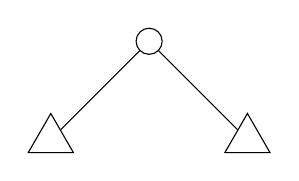
\begin{tikzpicture} [nodes=draw,
triangle/.style = {regular polygon, regular polygon sides=3 }
]
\node[circle](r){};
\node[triangle, below left = of r] (a) {};
\node[triangle, below right = of r] (b) {};
\draw (r) -- (a);
\draw (r) -- (b);
\end{tikzpicture}
%Finally, if you have citations, see the commented-out stuff in the \LaTeX~here.

%\

%My farourive Optimization books are \cite{bertsimas1997introduction} \cite{boyd2004convex} \cite{wolsey2014integer}. You should add bibliographical notes in the \textbf{BibTex}: \textit{mybib.bib} file. Its good to grab these notes from Google scholar citations.

%%%%%%%%%% If you don't have citations then comment the lines below:

%\bibliographystyle{abbrv}           % if you need a bibliography
%\bibliography{mybib}                % assuming yours is named mybib.bib

%%%%%%%%%%% end of doc
\end{document}
